% ============================================================
%  HOMEWORK REPORT TEMPLATE
%  Compile with: pdflatex homework_template.tex
% ============================================================
\documentclass[11pt, letterpaper]{article}

% ── Packages ────────────────────────────────────────────────
\usepackage[margin=1in]{geometry}
\usepackage{fancyhdr}
\usepackage{hyperref}
\usepackage{amsmath, amssymb}
\usepackage{enumitem}
\usepackage{booktabs}
\usepackage{xcolor}
\usepackage{setspace}
\usepackage{array}
\usepackage{graphicx}
\usepackage{subcaption}
\usepackage{multirow}
\usepackage{tabularx}
\usepackage{colortbl}
\usepackage{float}
\usepackage{placeins}
\usepackage{chngcntr}
\usepackage{lastpage}

% Load amsthm BEFORE parskip and titlesec to avoid patch conflict
\usepackage{amsthm}
\usepackage{parskip}

\usepackage{background}
\backgroundsetup{
  scale=8,
  angle=45,
  opacity=0.1,
  color=gray,
  contents={JSCHROEDER39}
}

\usepackage{titlesec}

\allowdisplaybreaks
\counterwithin*{equation}{subsection}

% ── Hyperlink Styling ────────────────────────────────────────
\hypersetup{
    colorlinks   = true,
    linkcolor    = black,
    urlcolor     = blue,
    citecolor    = black,
    pdftitle     = {Project Proposal},
}

% ── Header / Footer Setup ───────────────────────────────────
\pagestyle{fancy}
\fancyhf{}
\setlength{\headheight}{15pt}

\lhead{\textbf{\CourseName}}

\rhead{\AssignmentName}
\renewcommand{\headrulewidth}{1.2pt}
\cfoot{\thepage}
\renewcommand{\footrulewidth}{0pt}

% ── User-Defined Information ─────────────────────────────────
\newcommand{\StudentName}{Jacob Schroeder}
\newcommand{\TeamNumber}{42}
\newcommand{\CourseName}{ISYE6740: Computational Data Analysis}
\newcommand{\AssignmentName}{Final Report}
\newcommand{\AssignmentDue}{July 31, 2026}

% ── Section Formatting ──────────────────────────────────────
% Section: large bold, numbered "1.", rule beneath
\titleformat{\section}
    {\large\bfseries}
    {\thesection.}
    {0.5em}
    {}
    

% Subsection: normal size bold, numbered "1.1"
\titleformat{\subsection}
    {\normalsize\bfseries}
    {\thesubsection}
    {0.5em}
    {}

% ── Table of Contents Depth ─────────────────────────────────
\setcounter{tocdepth}{2}

% ============================================================
\begin{document}

% ── COVER PAGE ──────────────────────────────────────────────
\thispagestyle{empty}
\begin{center}
    \vspace*{1.5cm}

    {\Huge \textbf{\AssignmentName}}\\[0.6cm]
    {\large \CourseName}\\[0.4cm]
    \rule{0.6\textwidth}{0.8pt}\\[0.8cm]

    \begin{tabular}{>{\bfseries}r l}
        Name:        & \StudentName   \\[4pt]
        Team Number:  & \TeamNumber     \\[4pt]
        Due Date:    & \AssignmentDue \\[4pt]
    \end{tabular}

    \vspace{1.2cm}
    \rule{0.6\textwidth}{0.8pt}
\end{center}

% ── TABLE OF CONTENTS ───────────────────────────────────────
\newpage
\thispagestyle{fancy}
\tableofcontents

% ============================================================
%  REPORT BEGIN HERE
% ============================================================

\newpage
\section{Introduction}

LEGO has a fascinating history. Originating in Denmark in 1932, it began as a small wooden toy manufacturer. Since then it has grown into one of the most iconic toys ever produced. The LEGO brick as we know it today was introduced in 1958, and since then the brand has released thousands of distinct sets spanning dozens of licensed and original themes. Everything from the earliest Town and Castle series released in the 1970s, to the endlessly popular Star Wars licensed sets released beginning in the late 1990s, to the adult-targeted Icons and Architecture lines released for those of us who haven't fully grown up yet each set comes with hundreds of individual parts, colors, minifigures and other characteristics that make it both distinct and part of a greater collection.

Over the years, LEGO sets have evolved in piece count, colors, set complexity, and other key changes that make LEGO what they are. Things like the first lego sets with instructions being introduced in 1964, LEGO Technic introducing an entirely new style of piece getting added in 1977, the first Start Wars licensed set released in 1999, and robotics getting added with LEGO Mindstorms in 2006 have all been critical additions which have shaped the brand and the composition of those sets. This project examines that composition and how it has changed over the years.

\section{Problem Statement}
\label{sec:problem_statement}

\textit{Can unsupervised machine learning detect meaninful structural shifts in LEGO set design over time, and do those detected shifts correspond to known historical events in the company's history?}

This is the question that this project answers using temporal clustering \cite{chi2007evolutionary} and distributional drift detection \cite{gama2014survey}. Over the past several decades, LEGO has expanded from a company focusing primarily on traditional building sets to a global entertainment brand ecompassing licensed franchises, collector-focused products, and highly specialized themes. These changes are incredibly well documented from a business perspective, but it can be very uncelar how LEGO's product designs have evolved over time when viewed solely through the characteristics of the sets. 

The objective of this project is to analyze the evolution of LEGO products from the 1950s through the present day using unsupervisded machine learning techniques. Specifically, LEGO sets will be grouped into clusters based on structural and design-related features and the analysis examines how these clusters change over time. When looking at the shifts in the composition of clusters across different years, the expectation is that certain substaintial changes will appear aligning with major changes to LEGO's product portfolio. 

Let $S = \{ s_1, s_2, ..., s_N\}$ denote the full catalog of official LEGO sets, those being the sets released for standard sale and not including any of the promotional materials, special editions, or subsets which are sold as larger groups. Each set $s_i$ is characterized by a feature vector $\mathbf{x}_i \in \mathbb{R}^d$ derived from its structural composition. Each set carries a release year $y_i \in \{1955, ..., 2026\}$. We partition $S$ into cohorts made up of one of more years, $C_t = \{s_i:y_i = t\}$ for each time period $t$.

There are two ideas at the core of this problem:

\begin{enumerate}
    \item \textbf{Temporal Clustering:} For each cohort $C_t$, this project fits a clustering model $K_t$ that partitions sets into $k$ groups based on structural similarity. The cluster centroids are tracked $\{\mu_1^{(t)},...,\mu_k^{(t)}\}$ for each period $t$.
    \item \textbf{Drift Detection:} Measuring the degree of distributional change between consecutive cohort clusterings $K_t$ and $K_{t+1}$ using a quantitative dissimilarity metrix. This will identify specific years, $t^*$, where this dissimilarity exceeds a threshold. These years will be noted as \textit{drift points}.
\end{enumerate}

A formal notation of the goal of this project is to estimate:

\[
\Delta_t = \text{drift}(K_t, K_{t+1}), \quad t \in \{1955, ..., 2026\}
\]

where $\text{drift}(K_t, K_{t+1})$ is the drift shown by clustering dissimilarity measured using centroid displacement and Adjusted Rand Index. A detected drift point is defined as:

\[
t^* = \{t:\Delta_t > \mu_{\Delta} + c \sigma_{\Delta}\}
\]

$c$ is a tunable threshold and $\mu_{\Delta}$ and $\sigma_{\Delta}$ are the mean and standard deviation of $\Delta_t$ across all years. 

The hypothesis is that drift points $t^*$ will cluster near known historical milestones in LEGO's product history. Some examples of this would be the introduction of the Star Wars license in 1999, the near bancruptcy of the company in $2003-2004$, the growth of licensed themes throughout the 2010s, and the growth of adult targetted sets in the 2020s. If these events can be detected using structural, label-free features this would constitute a meaningufl unsupervised result. 

\section{Methodology}

\subsection{Data Source and Preprocessing}

Data has been sourced from the Rebrickable database \cite{rebrickable2024}, which provides both API and CSV exports for all lego set related data. For this project, I used the CSV export of a large relational database including the following tables: \texttt{sets}, \texttt{themes}, \texttt{parts}, \texttt{part\_categories}, \texttt{colors}, \texttt{inventories}, \texttt{inventory\_parts}, \texttt{inventory\_minifigs}, and \texttt{minifigs}. The complete entity relationship diagram including all attributes can be found in Appendix~\ref{sec:appendix_erd}. These were loaded into a local SQLite database via Python's \texttt{sqlite3} module and queried using \texttt{pandas}. 

Sets with a very small number ($n < 20$) of parts were be excluded as well as non-standard releases (e.g., promotional packs, individual minifigures, individual parts sold as set, merchandise with set numbers). Additionally, years with a small number of sets released in the catalog were grouped using rolling windows to ensure a large enough cohort size for stable clustering. Grouping was accomplished by setting a minimum cohort size (100) along with a maximum number of years per cohort (12). This ensured sufficient cohort size while not allowing for too many years to be clustered. Years with more than the minimum cohort size were evaluated alone. 

\subsection{Feature Engineering}

Each set $s_i$ is represented by a $d$-dimensional feature vector spanning four categories: scale (total part count, unique part count, minifigure count, spare part ratio), diversity (Shannon entropy of part categories $H_\text{cat}$, Shannon entropy of colors $H_\text{col}$, number of distinct colors, number of distinct part categories), composition (proportion of Technic parts, proportion of decorative/printed parts, proportion of transparent parts via \texttt{colors.is\_trans}, rare part ratio for parts appearing in fewer than 20 sets), and minifigure characteristics (minifigure-to-part ratio, a binary indicator for minifigure presence).

Before modeling, I screened this candidate set for multicollinearity using Variance Inflation Factors (Table \ref{tab:vif_original}). Two features stood out immediately: \texttt{total\_part\_count} and \texttt{num\_parts} had VIF values above 7000, reflecting their near-total redundancy, and \texttt{n\_distinct\_categories} exceeded the common threshold of 10. We removed both \texttt{total\_part\_count} and \texttt{n\_distinct\_categories} and recomputed VIF on the remaining twelve features (Table \ref{tab:vif_reduced}); all values fell below 5, indicating the reduced set carries largely independent information.

\begin{table}[h]
\centering
\caption{Variance Inflation Factors (Original Feature Set)}
\label{tab:vif_original}
\begin{tabular}{clr}
\hline
\textbf{\#} & \textbf{Feature} & \textbf{VIF} \\
\hline
0  & num\_parts              & 8299.992733 \\
1  & total\_part\_count       & 8145.789045 \\
2  & unique\_part\_count      & 13.160328 \\
3  & minifig\_count          & 5.305488 \\
4  & spare\_part\_ratio       & 1.297114 \\
5  & h\_cat                  & 5.350565 \\
6  & h\_col                  & 3.749628 \\
7  & n\_distinct\_colors      & 7.882505 \\
8  & n\_distinct\_categories  & 15.857922 \\
9  & prop\_technic           & 1.231668 \\
10 & prop\_printed           & 1.929013 \\
11 & prop\_transparent       & 1.186414 \\
12 & rare\_part\_ratio        & 2.373186 \\
13 & minifig\_to\_part\_ratio  & 1.317496 \\
14 & has\_minifigs           & 2.428044 \\
\hline
\end{tabular}
\end{table}

\begin{table}[h]
\centering
\caption{Variance Inflation Factors (Reduced Feature Set)}
\label{tab:vif_reduced}
\begin{tabular}{clr}
\hline
\textbf{\#} & \textbf{Feature} & \textbf{VIF} \\
\hline
0  & num\_parts              & 2.904824 \\
1  & unique\_part\_count      & 4.509105 \\
2  & minifig\_count          & 1.952869 \\
3  & spare\_part\_ratio       & 1.245666 \\
4  & h\_cat                  & 2.159906 \\
5  & h\_col                  & 1.521950 \\
6  & prop\_technic           & 1.224180 \\
7  & prop\_printed           & 1.924807 \\
8  & prop\_transparent       & 1.185894 \\
9  & rare\_part\_ratio        & 2.363765 \\
10 & minifig\_to\_part\_ratio  & 1.286617 \\
11 & has\_minifigs           & 2.123624 \\
\hline
\end{tabular}
\end{table}

The retained twelve features still span the same three functional roles: scale and part diversity (\texttt{num\_parts}, \texttt{unique\_part\_count}), minifigure presence and intensity (\texttt{minifig\_count}, \texttt{has\_minifigs}, \texttt{minifig\_to\_part\_ratio}), and material or stylistic composition (\texttt{h\_cat}, \texttt{h\_col}, \texttt{prop\_technic}, \texttt{prop\_printed}, \texttt{prop\_transparent}, \texttt{rare\_part\_ratio}, \texttt{spare\_part\_ratio}). Rather than relying on piece count alone, this combination captures how a set is built. Each feature is normalized prior to clustering. Note that this VIF-reduced set is used only for the UMAP visualization described in Section~\ref{sec:umap}; the temporal clustering described in Section~\ref{sec:temporal_clustering} uses the full feature set, since collinearity among features is less consequential for distance-based clustering methods like $k$-means than it is for interpreting a low-dimensional projection.

\subsection{Dimensionality Reduction for Visualization}
\label{sec:umap}

To visualize the structure of the feature space described above, I applied Uniform Manifold Approximation and Projection (UMAP) \cite{mcinnes2018umap} to the normalized feature matrix. UMAP was chosen over alternatives such as PCA or $t$-SNE for its ability to preserve both local neighborhood structure and, to a reasonable extent, global relationships between clusters, while remaining computationally efficient on the dataset size. I used a neighborhood size of $n_{\text{neighbors}} = 15$ and minimum distance of $0.1$, projecting the data into two components for the primary visualization and three components as a check on whether additional structure emerges beyond what is visible in two dimensions.

Figure \ref{fig:umap_2d} shows the resulting two-dimensional embedding, with points colored by time window to indicate when each set was released. The embedding reveals three to four well-separated clusters, along with a small number of isolated outlier points at the periphery. This separation indicates that the feature set captures genuinely distinct regimes of LEGO sets, likely corresponding to differences in theme, set type, or piece composition, that do not blend continuously into one another.

\begin{figure}[h]
    \centering
    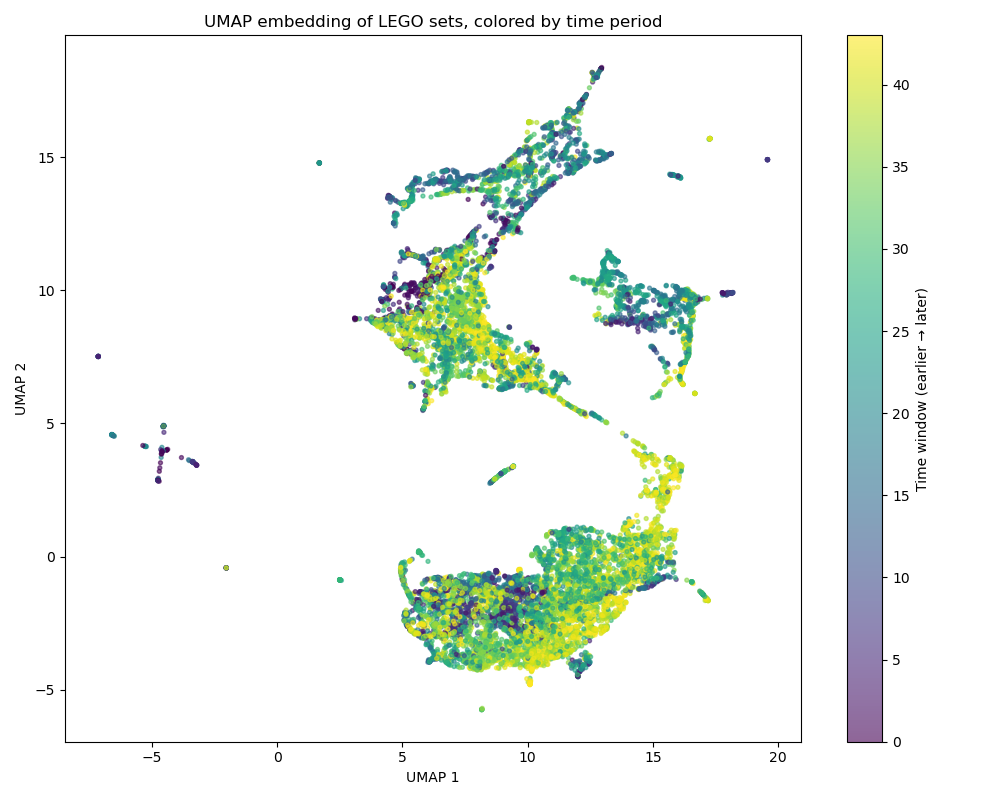
\includegraphics[width=0.8\textwidth]{Code/outputs/UMAP_embedding.png}
    \caption{Two-dimensional UMAP embedding of LEGO sets, colored by time window.}
    \label{fig:umap_2d}
\end{figure}

Notably, time window color is thoroughly mixed within each cluster rather than segregated: early and late sets of a given type occupy the same region of the embedding. This suggests that time of release is not the dominant axis separating set types, since a strong time effect would appear as solid-colored blobs rather than mixed ones. A weaker secondary time trend is still visible, however: later sets tend to concentrate toward the outer edges of each cluster, while earlier sets sit closer to the center, implying that set characteristics drift gradually over time within a given type even though type itself is the primary driver of cluster membership.

The embedding also exhibits several thin tendrils connecting or extending from the main clusters. These likely correspond to sets that are transitional between two categories, or to sparsely represented set variants such as reissues. Identifying which sets populate these bridging regions is a natural next step for validating the semantic meaning of the clusters.

To confirm that two dimensions are sufficient to capture the dominant structure, I repeated the embedding with three components and inspected it from multiple viewing angles (Figure \ref{fig:umap_3d} in Appendix~\ref{sec:appendix_umap}). The three-dimensional projection reproduces the same three-cluster structure and the same within-cluster mixing of time windows observed in two dimensions, with no additional cluster or separation emerging along the third axis. This indicates that the two-dimensional embedding is not discarding meaningful structure, and that two components are adequate for downstream visualization and interpretation.

\subsection{Temporal Clustering}
\label{sec:temporal_clustering}

The optimal number of clusters $k$ is selected using the elbow method and silhouette score analysis on the second-to-last cohort rather than the most recent one. The final cohort in the dataset does not correspond to a complete year, since it captures only the partial set of releases available at the time of data collection, whereas the second-to-last cohort corresponds to 2025, the most recent complete year of releases. Selecting $k$ from a full year avoids anchoring the clustering solution to an incomplete and potentially unrepresentative sample. Cluster fitting itself proceeds backward in time, beginning from this reference cohort and moving through earlier cohorts, so that each earlier cohort's structure is interpreted relative to present-day design conventions rather than relative to the earliest sets in the catalog. Drift, by contrast, is calculated moving forward through time: $\Delta_t$ measures the change from cohort $t$ to cohort $t+1$, so that detected drift points $t^*$ correspond to the year in which a shift occurred, consistent with the historical framing in Section~\ref{sec:problem_statement}.

To address any concern that standard $k$-means clustering applied independently per cohort may produce inconsistent labeling (the ``cluster correspondence problem''), centroids were matched across consecutive years using the Hungarian algorithm to minimize total centroid displacement \cite{kuhn1955hungarian}.

\subsection{Robustness Check via DBSCAN}

As a robustness check on the $k$-means-based temporal clustering, I will additionally fit DBSCAN \cite{ester1996dbscan} to each cohort $\mathcal{C}_t$. Unlike $k$-means, DBSCAN does not require a fixed number of clusters to be specified in advance and can identify clusters of arbitrary shape, while explicitly labeling low-density points as noise rather than forcing them into the nearest cluster. This makes it a useful check on two assumptions underlying the primary $k$-means approach: first, that the fixed value of $k$ selected from the 2025 reference cohort remains an appropriate choice across earlier cohorts with potentially different underlying structure, and second, that LEGO sets naturally form roughly spherical, similarly sized groups in feature space, an assumption implicit in $k$-means but not required by DBSCAN. Rather than treating DBSCAN as a competing model to be scored against $k$-means, its purpose here is diagnostic: if DBSCAN, run independently and without the constraint of a fixed $k$, recovers a broadly similar number and shape of clusters within each cohort, this lends confidence that the cluster structure detected by $k$-means reflects genuine groupings in the data rather than an artifact of its shape assumptions. If DBSCAN instead reveals substantially different structure, particularly within cohorts flagged as drift points, this would signal that conclusions drawn from the $k$-means clustering warrant additional caution rather than invalidating them outright.

\subsection{Drift Detection}

The dissimilarity between consectuive clustering solutions were measured using two metrics:

\begin{enumerate}
    \item \textbf{Adjusted Rand Index (ARI):} For sets present in both cohorts $\mathcal{C}_t$ and $\mathcal{C}_{t+1}$ (overlapping years), ARI will measure the agreement between the two clustering assignments. A sharp drop in ARI signals structural reorganization \cite{mishra2025cluster}.
    \item \textbf{Centroid displacement:} The average Euclidean distance between matched centroid pairs $\|\mu_j^{(t+1)} - \mu_j^{(t)}\|_2$, averaged over all $k$ clusters, captures smooth directional drift even when set membership does not overlap between cohorts.
\end{enumerate}

\subsection{Reproducibility}

All code has been written in Python and made available alongside the SQLite database construction scripts. Random seeds were fixed at 42 (the meaning of life, the universe, and everything) to ensure reproducible random cluster initializations. 

\noindent\rule{\textwidth}{0.4pt}

\section{Evaluation Strategies}

\subsection{Internal Clustering Validity}

For each annual clustering solution $\mathcal{K}_t$, internal quality will be assessed using:
\begin{itemize}
    \item \textbf{Silhouette score:} Measures how similar each point is to its own cluster relative to other clusters; scores near $1$ indicate well defined clusters \cite{rousseeuw1987silhouettes}.
    \item \textbf{Davies-Bouldin Index:} Penalizes clusters that are large and close together; lower values indicate better separation.
    \item \textbf{Elbow method on inertia:} Confirms that the chosen $k$ is appropriate and stable across years.
\end{itemize}

Consistency of these metrics across years will itself be informative: a sudden degradation in silhouette score in a given year suggests the data no longer conforms to the assumed cluster geometry, which is an independent signal of drift.

\subsection{External Validation Against Theme Labels}

Although theme labels are not used as features, they can be used for external validations. After fitting each annual clustering, I will compute:
\begin{itemize}
    \item \textbf{Normalized Mutual Information (NMI)} between cluster assignments and official theme labels
    \item \textbf{Homogeneity and completeness scores} to assess whether clusters align with the theme.
\end{itemize}

\section{Conclusion}

LEGO has long been a passion of mine from a very young age. While my appreciationn for the brand and the product began as a child, it has remained a hobby well into adulthood. My growth reflects LEGOs growth. When I was younger, I thought that LEGO Star Wars was the greatest thing on earth. While I still love those sets, my passions have shifted towards the large-scale car models like the Formula 1 cars, Porsche 911, Land Rover Defender, as well as the new LEGO Lord of the Rings collection.

This project gives me a great opportunity to combine a personal passion for LEGO with the machine learning techniques studied in this course. By applying clustering and drift detection methods to decades of LEGO set data, I hope to uncover patterns in the evolution of the brand and show how the composition of the product design which has made this iconic brand so successful reveals shifts not obvious to the human eye.

\newpage

\appendix
\section{Appendix}

\subsection{Rebrickable Entity Relationship Diagram}
\label{sec:appendix_erd}

\begin{figure}[h]
  \centering
  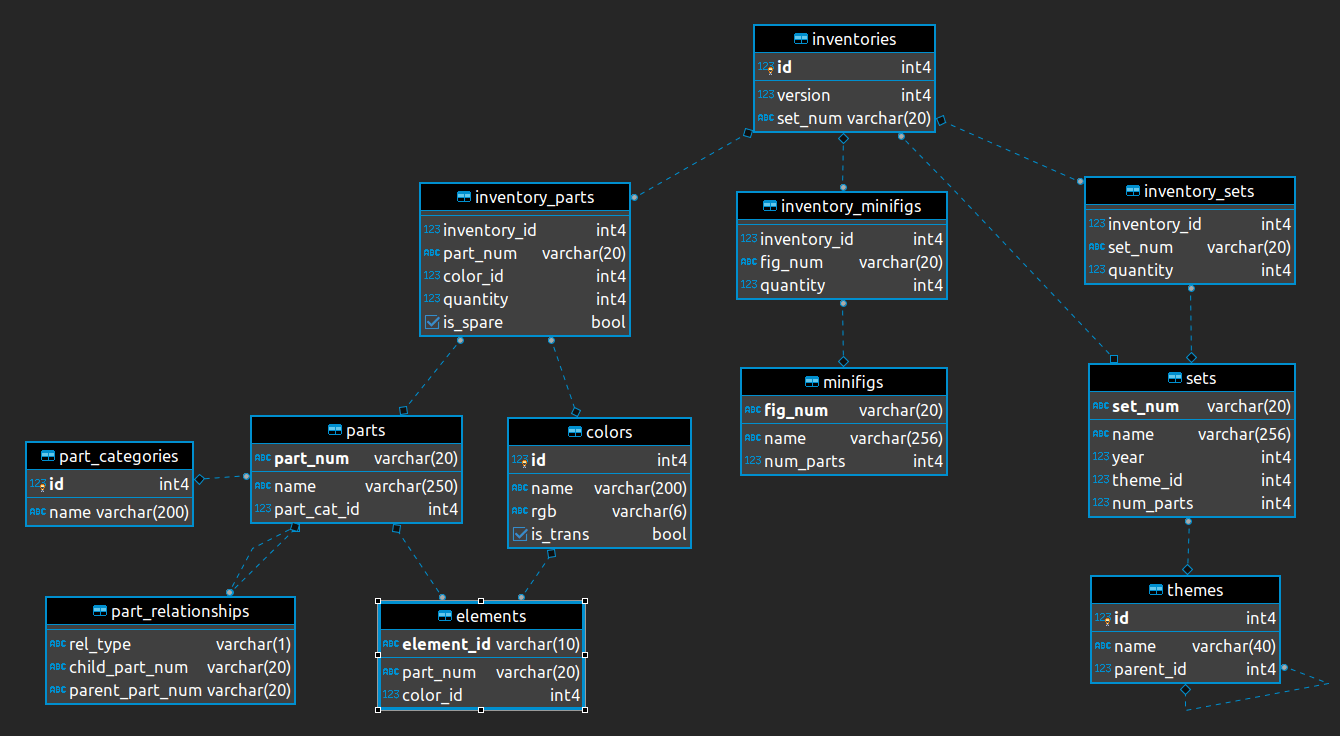
\includegraphics[width=1\textwidth]{images/ERD.png}
    \caption{Database schema for the Rebrickable \cite{rebrickable2024} LEGO dataset. The relational structure links LEGO sets to inventories, parts, colors, themes, and minifigures, providing the foundation for feature engineering and longitudinal analysis of changes in LEGO product design over time.}
    \label{fig:erd}
\end{figure}

\FloatBarrier

\newpage

\subsection{Breakdown of Number of Sets per Time Window}
\label{sec:appendix_windows}

\begin{table}[h]
\centering
\caption{Number of Sets per Time Window}
\label{tab:sets_per_window}
\begin{tabular}{crrr@{\hspace{1.5em}}crrr}
\hline
\textbf{Window} & \textbf{num sets} & \textbf{min} & \textbf{max} & \textbf{Window} & \textbf{num sets} & \textbf{min} & \textbf{max} \\
\hline
0  & 56  & 1955 & 1966 & 22 & 227 & 2005 & 2005 \\
1  & 131 & 1967 & 1973 & 23 & 216 & 2006 & 2006 \\
2  & 110 & 1974 & 1976 & 24 & 209 & 2007 & 2007 \\
3  & 149 & 1977 & 1979 & 25 & 238 & 2008 & 2008 \\
4  & 101 & 1980 & 1981 & 26 & 272 & 2009 & 2009 \\
5  & 137 & 1982 & 1984 & 27 & 252 & 2010 & 2010 \\
6  & 104 & 1985 & 1985 & 28 & 311 & 2011 & 2011 \\
7  & 219 & 1986 & 1987 & 29 & 358 & 2012 & 2012 \\
8  & 134 & 1988 & 1989 & 30 & 362 & 2013 & 2013 \\
9  & 178 & 1990 & 1991 & 31 & 423 & 2014 & 2014 \\
10 & 179 & 1992 & 1993 & 32 & 471 & 2015 & 2015 \\
11 & 105 & 1994 & 1994 & 33 & 496 & 2016 & 2016 \\
12 & 130 & 1995 & 1995 & 34 & 475 & 2017 & 2017 \\
13 & 139 & 1996 & 1996 & 35 & 487 & 2018 & 2018 \\
14 & 181 & 1997 & 1997 & 36 & 479 & 2019 & 2019 \\
15 & 276 & 1998 & 1998 & 37 & 496 & 2020 & 2020 \\
16 & 230 & 1999 & 1999 & 38 & 521 & 2021 & 2021 \\
17 & 265 & 2000 & 2000 & 39 & 508 & 2022 & 2022 \\
18 & 232 & 2001 & 2001 & 40 & 532 & 2023 & 2023 \\
19 & 250 & 2002 & 2002 & 41 & 610 & 2024 & 2024 \\
20 & 269 & 2003 & 2003 & 42 & 640 & 2025 & 2025 \\
21 & 250 & 2004 & 2004 & 43 & 452 & 2026 & 2026 \\
\hline
\end{tabular}
\end{table}

Number of sets per time window. Each window aggregates one or more consecutive release years to balance sample sizes across the dataset's history; \textbf{Window} is the window index, \textbf{num sets} is the count of LEGO sets falling in that window, and \textbf{min}/\textbf{max} give the first and last release year included in the window.


\FloatBarrier

\newpage

\subsection{Additional UMAP Visualizations}
\label{sec:appendix_umap}

This appendix presents supplementary UMAP visualizations that support the discussion in Section~\ref{sec:umap} (dimensionality reduction for visualization).

\begin{figure}[htbp]
    \centering
    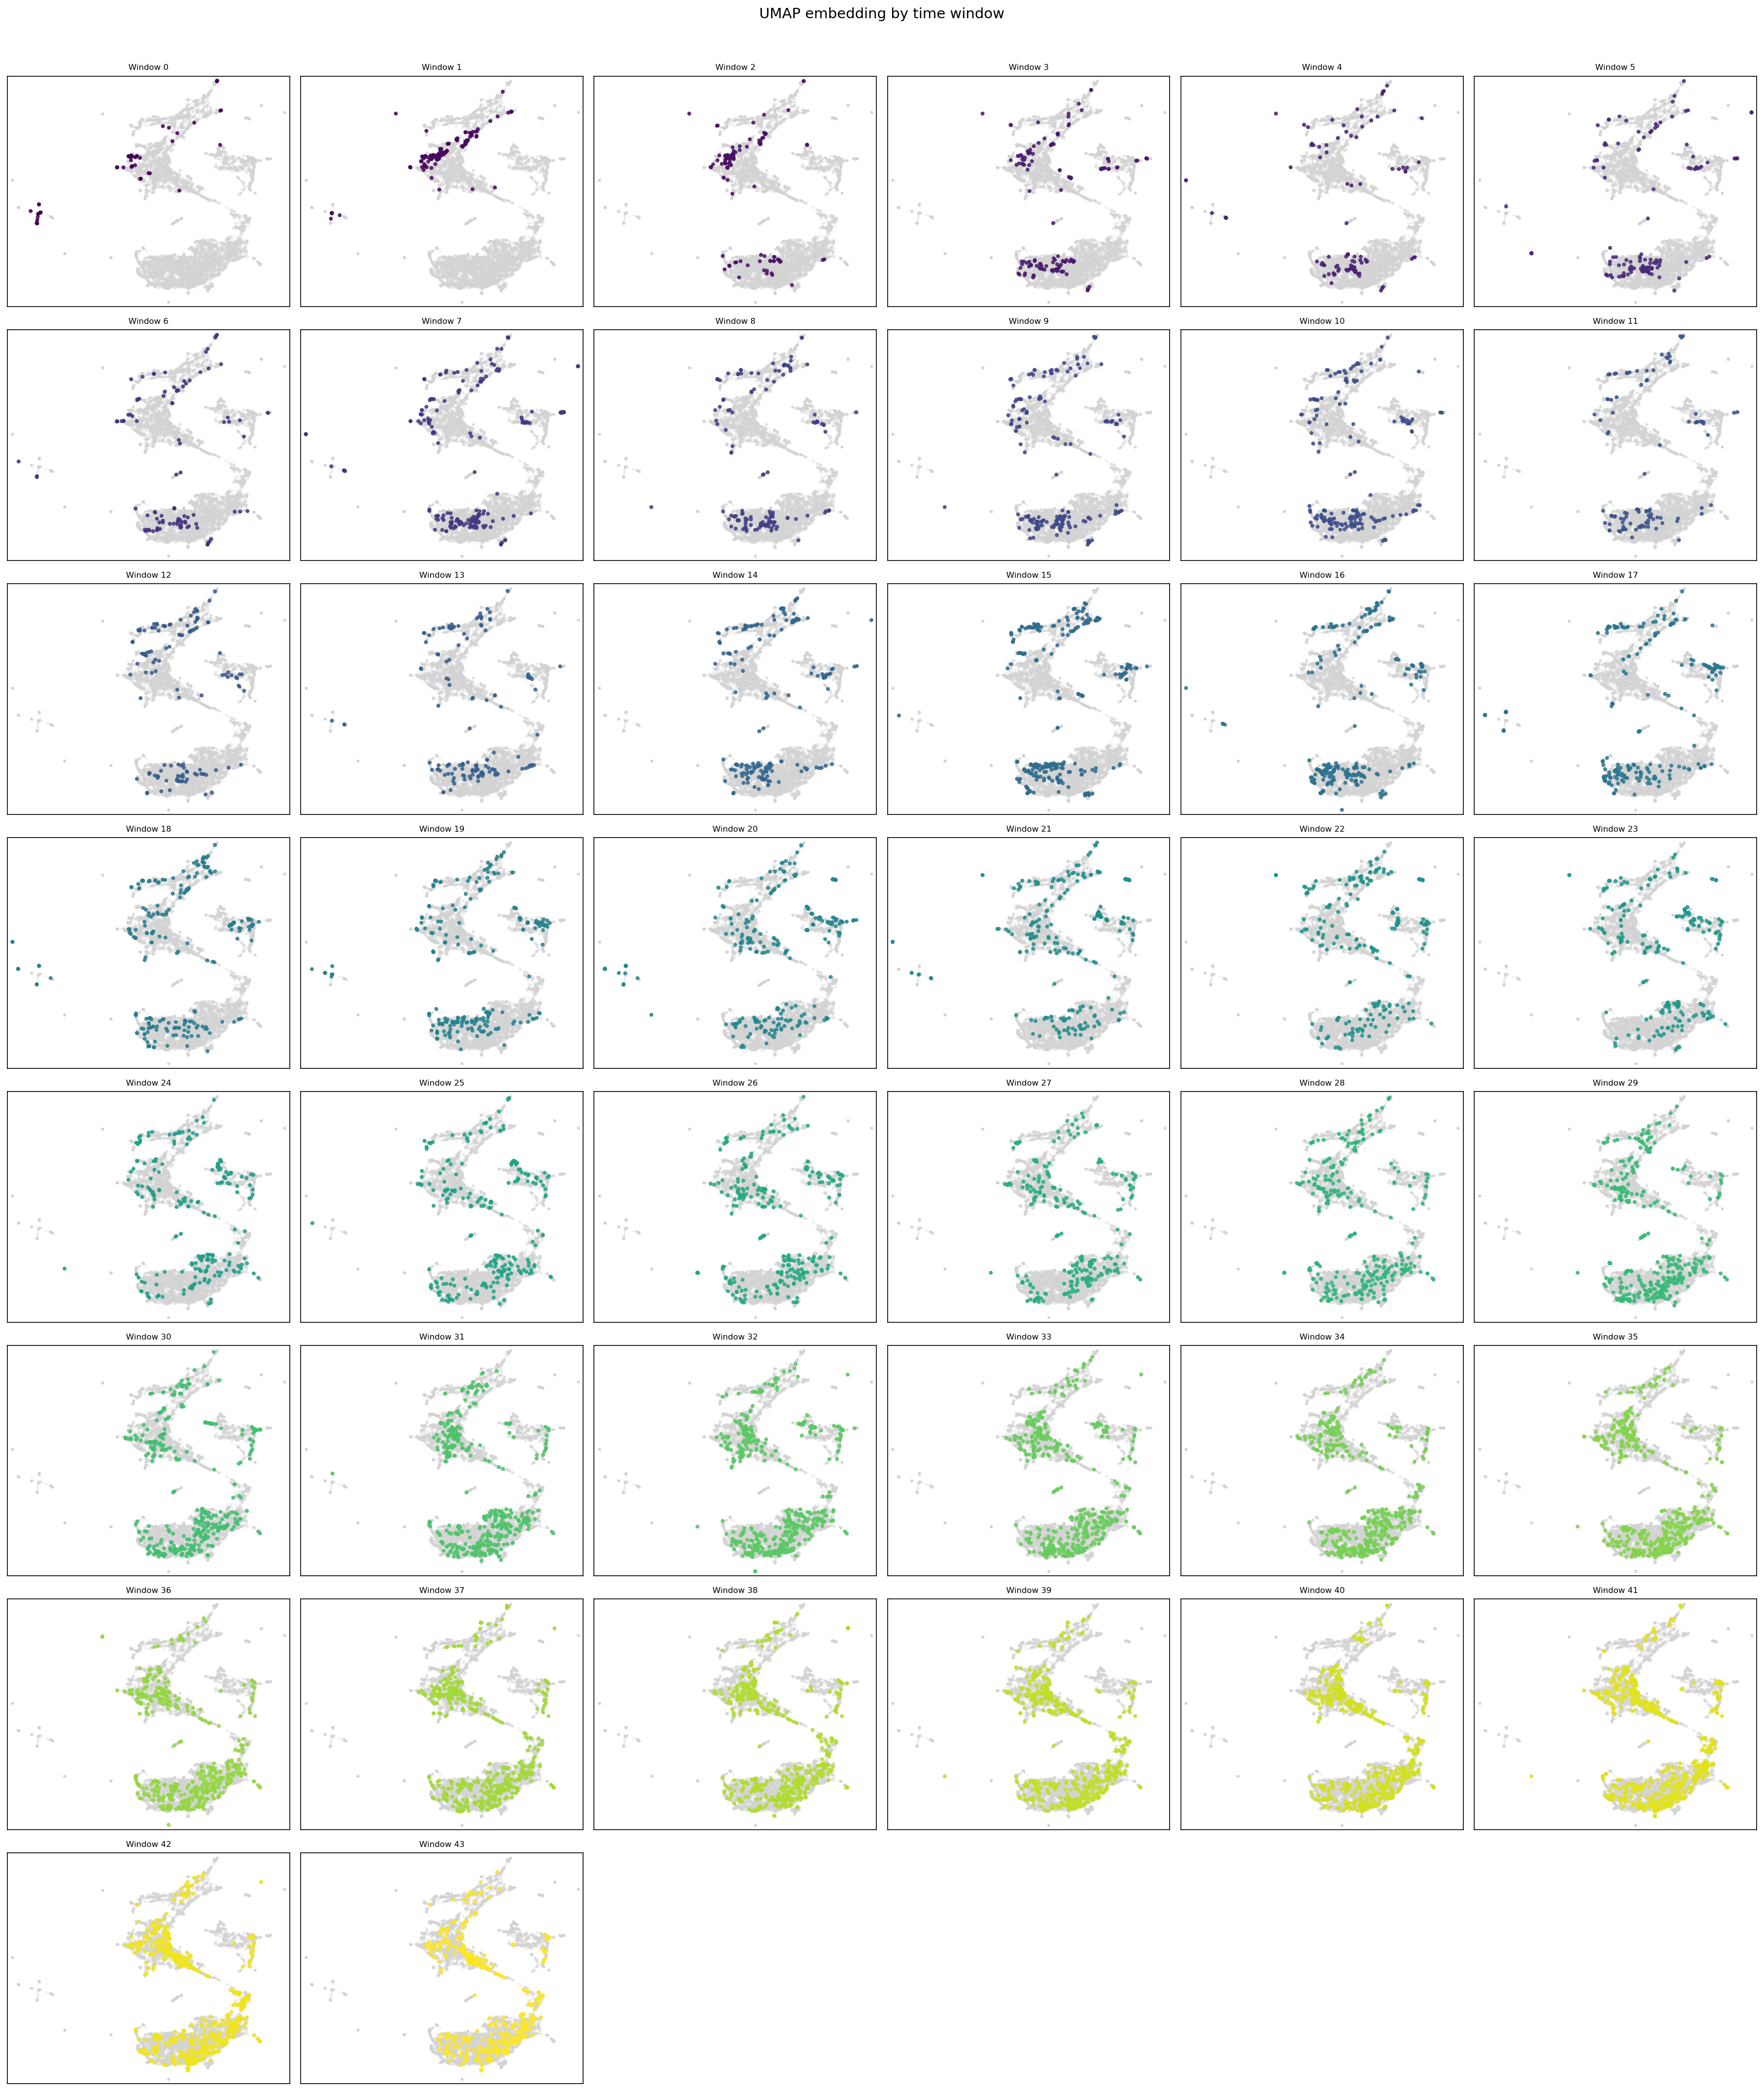
\includegraphics[width=.8\textwidth]{Code/outputs/UMAP_grid_by_window.png}
    \caption{Two-dimensional UMAP embedding faceted by time window. In each panel, points from that window are highlighted in color and all other points are shown in gray for reference.}
    \label{fig:umap_facet}
\end{figure}

Figure~\ref{fig:umap_facet} shows the same two-dimensional embedding as Figure~\ref{fig:umap_2d}, but faceted by individual time window rather than using a single continuous color scale. In each panel, points belonging to that window are highlighted in color while all other points are shown in gray for reference. This view makes the temporal drift within clusters easier to inspect than a single overlaid plot. In the earliest windows (0 through roughly 5), highlighted points are concentrated almost entirely in a small region of the upper cluster, indicating that sets released in this period are compositionally similar to one another and represent a narrow slice of the overall feature space. Moving through the middle windows, the highlighted region expands and begins to populate the lower cluster as well, suggesting the introduction of new set types over time rather than a simple continuation of earlier patterns. By the later windows (roughly 30 onward), highlighted points spread across nearly the full extent of both major clusters, indicating that recent sets span a much broader range of the feature space than earlier ones. This progressive broadening is consistent with the interpretation in Section~\ref{sec:umap} that set diversity, in terms of scale, composition, and minifigure content, has increased over time, even though time window itself is not the primary axis separating the clusters.

Figure~\ref{fig:umap_3d} shows the three-dimensional UMAP embedding from multiple viewing angles, used to confirm that no additional cluster structure is hidden along a third dimension beyond what is visible in the two-dimensional embedding.

\begin{figure}[htbp]
    \centering
    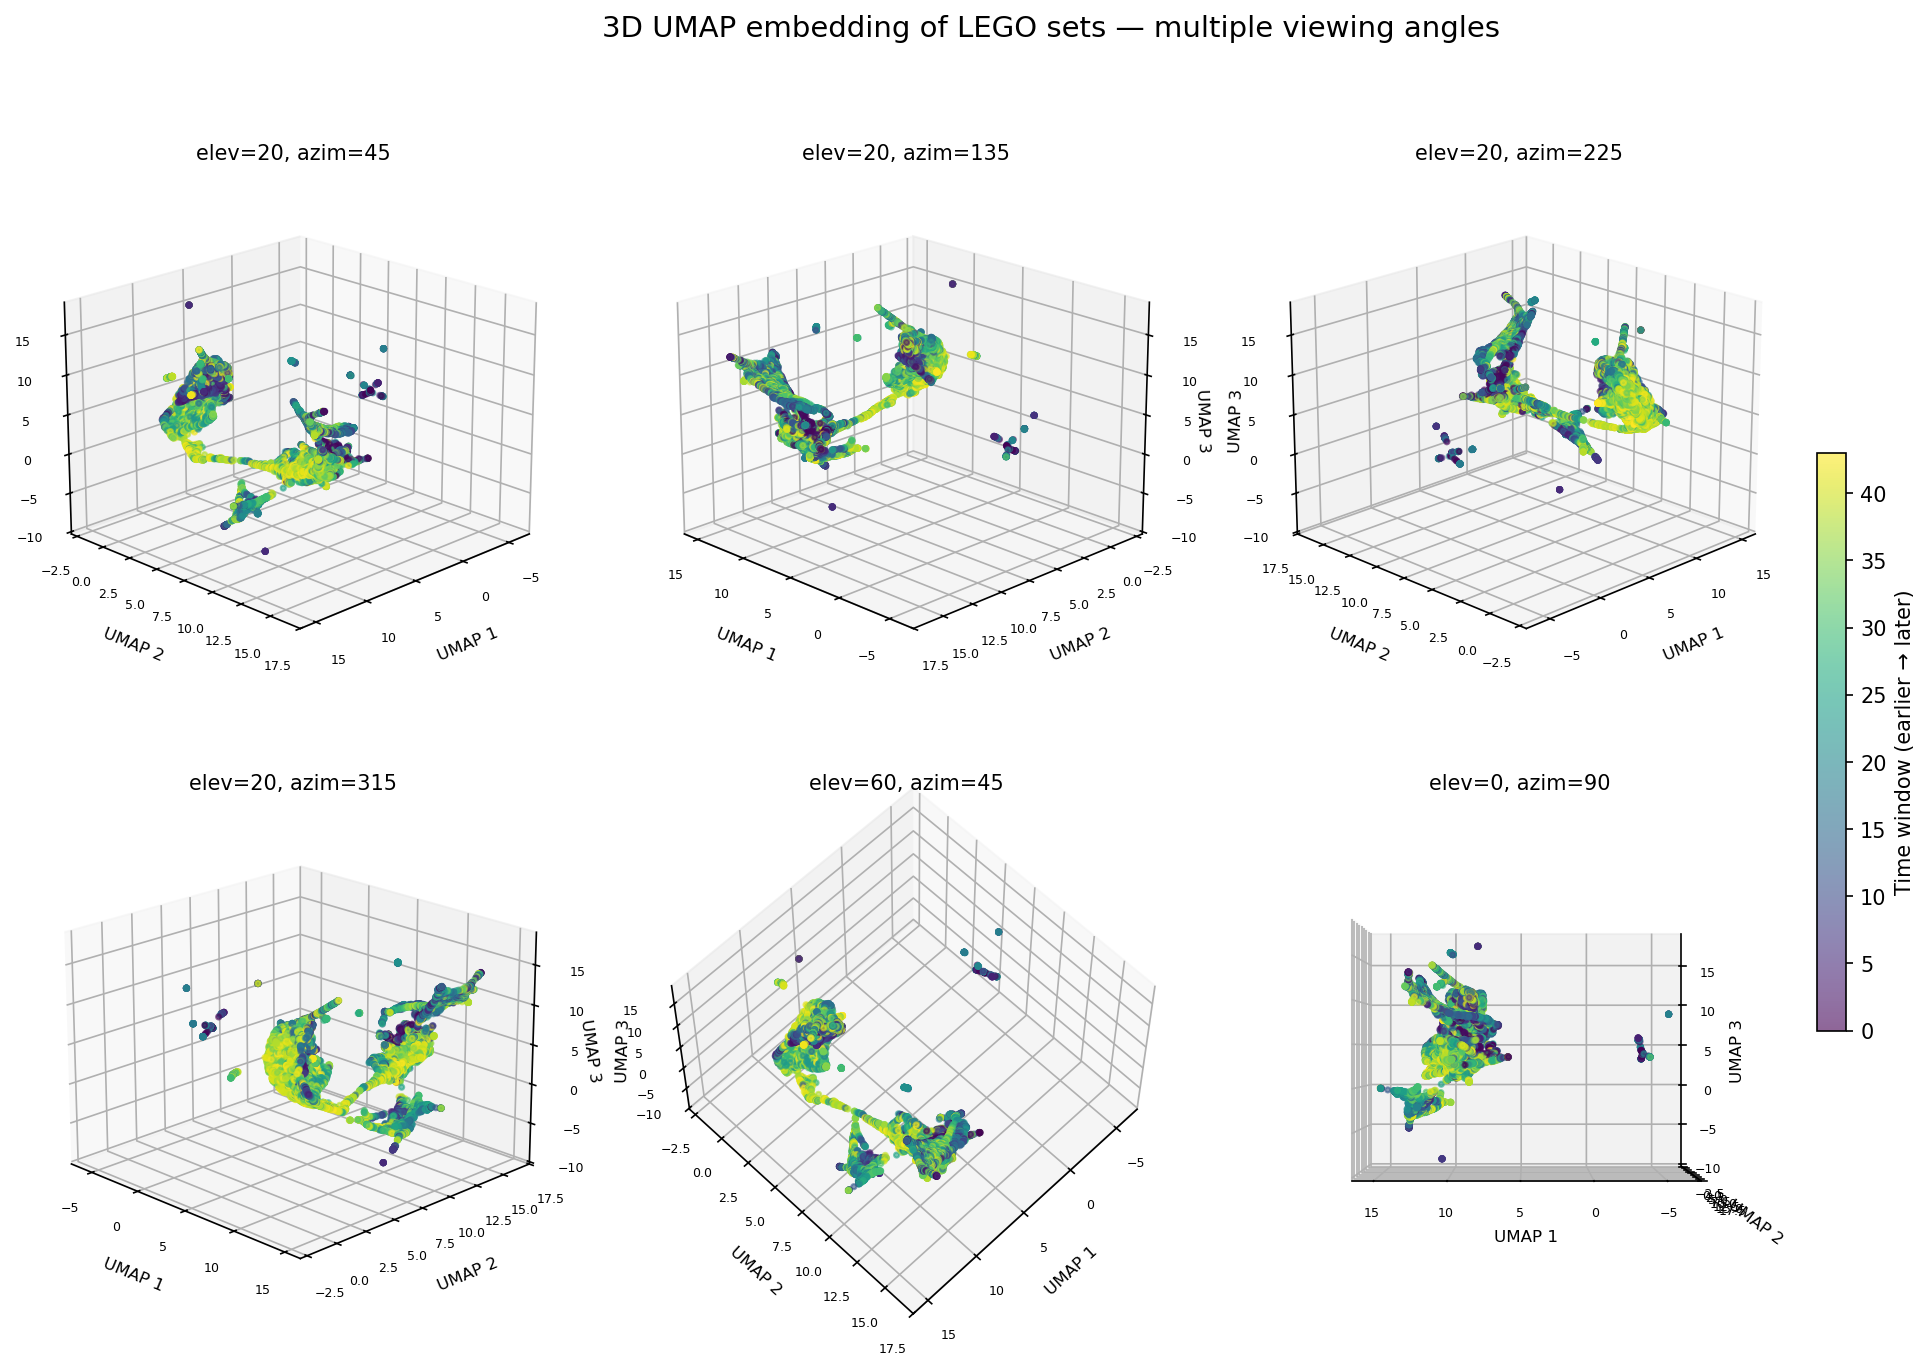
\includegraphics[width=\textwidth]{Code/outputs/UMAP_embedding_3d_multiangle.png}
    \caption{Three-dimensional UMAP embedding of LEGO sets viewed from multiple angles, colored by time window.}
    \label{fig:umap_3d}
\end{figure}

\FloatBarrier

\newpage

\addcontentsline{toc}{section}{References}

\begin{thebibliography}{9}

\bibitem{chi2007evolutionary}
Chi, Y., Song, X., Zhou, D., Hino, K., \& Tseng, B. L. (2007).
\newblock Evolutionary spectral clustering by incorporating temporal smoothness.
\newblock In \textit{Proceedings of the 13th ACM SIGKDD International Conference on Knowledge Discovery and Data Mining} (pp. 153--162).
\newblock \url{https://doi.org/10.1145/1281192.1281212}

\bibitem{ester1996dbscan}
Ester, M., Kriegel, H.-P., Sander, J., \& Xu, X. (1996).
\newblock A density-based algorithm for discovering clusters in large spatial databases with noise.
\newblock In \textit{Proceedings of the Second International Conference on Knowledge Discovery and Data Mining (KDD-96)} (pp. 226--231). AAAI Press.

\bibitem{gama2014survey}
Gama, J., Žliobaitė, I., Bifet, A., Pechenizkiy, M., \& Bouchachia, A. (2014).
\newblock A survey on concept drift adaptation.
\newblock \textit{ACM Computing Surveys}, 46(4), 1--37.
\newblock \url{https://doi.org/10.1145/2523813}

\bibitem{kuhn1955hungarian}
Kuhn, H. W. (1955).
\newblock The Hungarian method for the assignment problem.
\newblock \textit{Naval Research Logistics Quarterly}, 2(1--2), 83--97.
\newblock \url{https://doi.org/10.1002/nav.3800020109}

\bibitem{mcinnes2018umap}
McInnes, L., Healy, J., \& Melville, J. (2018).
\newblock UMAP: Uniform manifold approximation and projection for dimension reduction.
\newblock \textit{arXiv preprint arXiv:1802.03426}.
\newblock \url{https://arxiv.org/abs/1802.03426}

\bibitem{mishra2025cluster}
Mishra, A., \& Stamp, M. (2025).
\newblock Cluster analysis and concept drift detection in malware.
\newblock \textit{arXiv preprint arXiv:2502.14135}.
\newblock \url{https://arxiv.org/abs/2502.14135}

\bibitem{rebrickable2024}
Rebrickable. (2024).
\newblock LEGO sets database downloads.
\newblock \url{https://rebrickable.com/downloads/}

\bibitem{rousseeuw1987silhouettes}
Rousseeuw, P. J. (1987).
\newblock Silhouettes: A graphical aid to the interpretation and validation of cluster analysis.
\newblock \textit{Journal of Computational and Applied Mathematics}, 20, 53--65.
\newblock \url{https://doi.org/10.1016/0377-0427(87)90125-7}

\end{thebibliography}

\end{document}